\documentclass{article}
\usepackage[utf8]{inputenc, amsmath,titlesec,amssymb}
\usepackage[bottom]{footmisc}
\usepackage{graphicx}
\title{HW2}
\author{Freeman Chen}
\graphicspath{ {./images/} }


\begin{document}
\maketitle
\item{Question 1}


a. A * B = \begin{bmatrix}
5 & 5 & 5 \\
17 & 17 & 17 \\
12 & 12 & 12 \\
\end{bmatrix} (Matrix multiplication)


b. A * x = \begin{bmatrix} 
32\\
79\\
85
\end{bmatrix}(Matrix multiplication)

c. x'* B = \begin{bmatrix} 
17 & 17 & 17 \\
\end{bmatrix}(x transpose and Matrix multiplication)

d. B * y = error (B is a 3 by 3 matrix and y is a 1 by 3 matrix, we need the numbers of column of B match numbers of rows of y in order to run this function )

e. x * A = error ( x is a 3 by 1 matrix and A is a 3 by 3 matrix, we need the numbers of column of x match numbers of rows of A in order to run this function)

f. x * y = \begin{bmatrix}
15 & 50 & 45 \\
30 & 60 & 90 \\
40 & 80 & 120 \\
\end{bmatrix} (Matrix multiplication)

g. y * x = 195 (Matrix multiplication)

h. x * y' = error (x is a 3 by 1 matrix and y transpose is also a 3 by 1, so it not gonna work)

I. x .*y =  \begin{bmatrix}
15 & 50 & 45 \\
30 & 60 & 90 \\
40 & 80 & 120 \\
\end{bmatrix} (element multiplication)

J. A . *B = \begin{bmatrix}
2 & -1 & 4 \\
9 & 6 & 2 \\
1 & 3 & 8 \\
\end{bmatrix} (element multiplication)

\item{Question 2}

solution: 
x = \begin{bmatrix}
20  \\
-32 \\
13  \\
\end{bmatrix}\\

Rank of A = 3

I used 3 Method to solve the x, first, I used the linsolve function from matlab, second I use A\B, third I create an augmented matrix matrix and did the row reduced echelon form to find the solution

\item{Question 3}

I created a augmented matrix matrix and did the row reduced echelon form, and I get \begin{bmatrix}
1 & 0 & 0 \\
0 & 1 &0 \\
0 & 0 & 1 \\
\end{bmatrix}\\
which means there's no solution, the first two rows gave me $x_1 = 0, x_2 = 0$ but the third row gave me $x_1+x_2 = 1$ which is contradiction. therefor, there's no solution for this linear system, we can also see from the graph

\begin{figure}[h]
\centering

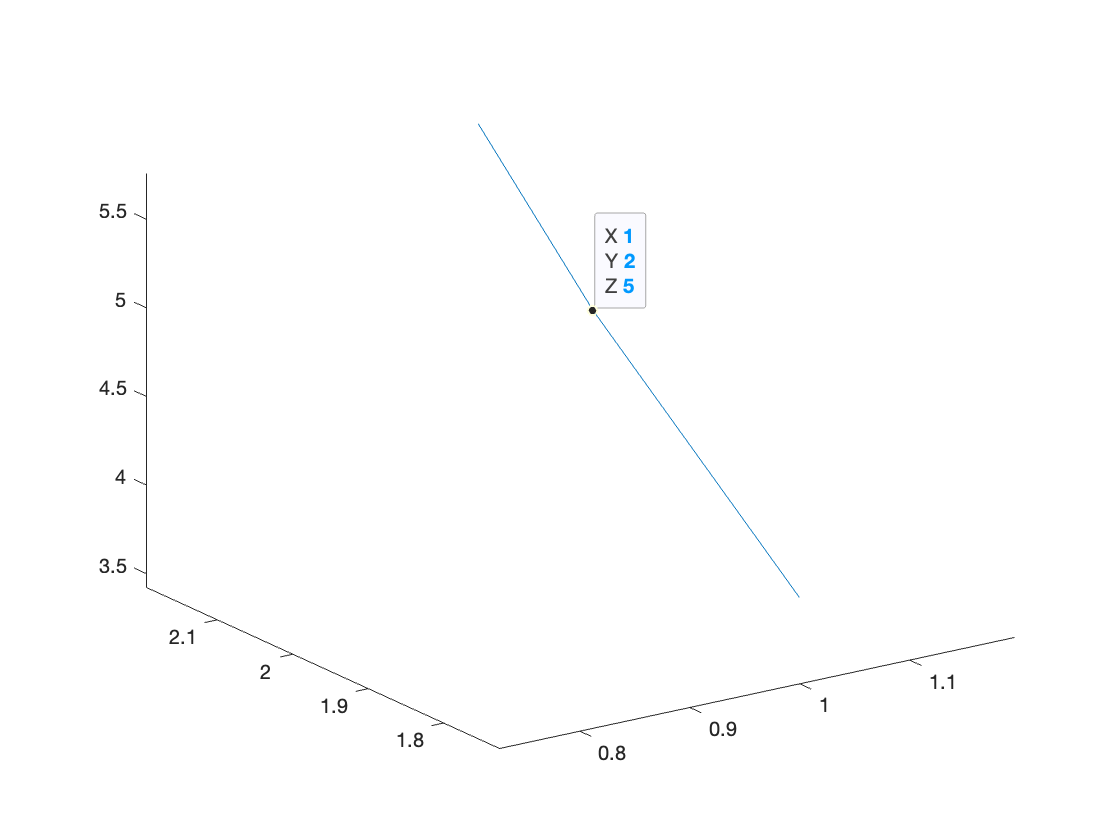
\includegraphics[width=0.5\textwidth]{HW2_3graph} \footnotemark[3] 

\end{figure}

\item{Question 4}

see github file @HW2_4

\item{Question 5}

\begin{figure}[h]
\centering

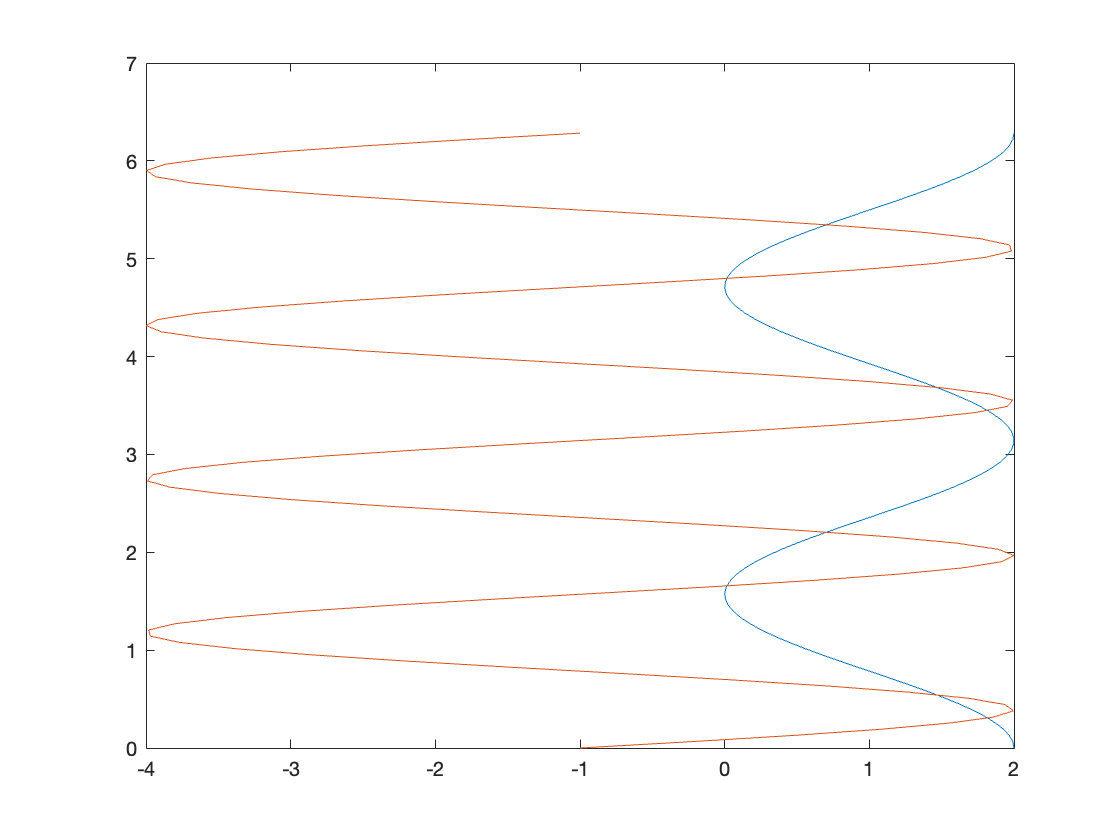
\includegraphics[width=0.5\textwidth]{Math300/images/parametric_curve.png} \footnotemark[3] 

\end{figure}


\end{document}